\documentclass{beamer}

% select theme
\usetheme{CambridgeUS}
\usecolortheme{beaver}

\usepackage{kotex}
\usepackage{fancyvrb}
\usepackage{color}
\usepackage[mmddyyyy]{datetime}
\usepackage{pythontex}
\usepackage{graphicx, subfigure}

% you need to generate pyg.tex by
% pygmentize -O full -f latex hello.c
% \input{pyg.tex}



% syntax highlighted source code 넣는법:
% http://ubuntuforums.org/showthread.php?t=790610
% pygmentize 명령어가 실행될 수 있도록 하자.
% bash에 그냥 pygmentize라고 치면 어느 패키지를 설치해야 하는지 알려줌.
% then...
% 색깔 명령어가 define될 수 있도록... hello.c를 만든 다음,
% pygmentize -O full -f latex hello.c
% 를 돌리면 무엇을 include해야 하는지, define이 뭐가 필요한지 쭉
% stdout으로 출력해줌.
% pygmentize -f latex hello.c 로 나오는 verbatim문을 긁어붙이면 완성.
\begin{document}

% title slide
\begin{frame}
	\title{딥러닝}
	\author{정민우}
	\date{\today}
	\titlepage
\end{frame}



% outline slide
\section*{Outline}
\begin{frame}
\tableofcontents
\end{frame}



\section{더 깊게}

% 그냥 글자만 있는 슬라이드
% \begin{frame}
% 	\begin{itemize}
% 		\item 합성곱 계층(Convolutional layer)
% 		\item 풀링 계층(Pooling layer)
% 	\end{itemize}
% \end{frame}
% 제목도 들어갔다.
\begin{frame}
	\frametitle{더 깊은 신경망으로}
	\begin{itemize}
		\item 층이 깊어질수록 채널 수가 늘어남
		\item 중간 데이터의 공간 크기는 줄어듬
		\item 드롭아웃 계층을 사용(Overfitting 방지)
		\item Adam을 이용해 최적화
		\item 가중치 초기값은 He 사용
	\end{itemize}
	\begin{figure}
		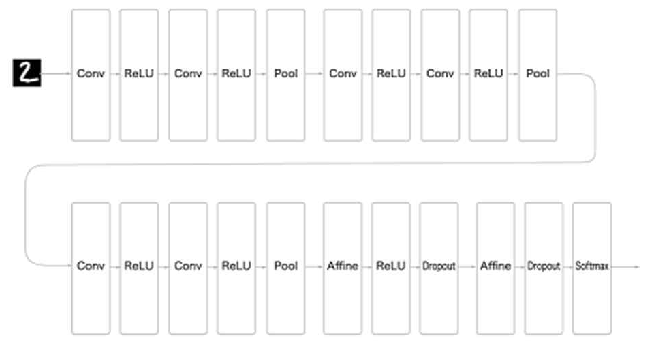
\includegraphics[width=0.5\columnwidth]{Fig_deep/Figure_1.pdf}
	\end{figure}
\end{frame}

\begin{frame}
	\frametitle{더 깊은 신경망으로}
	\begin{figure}
		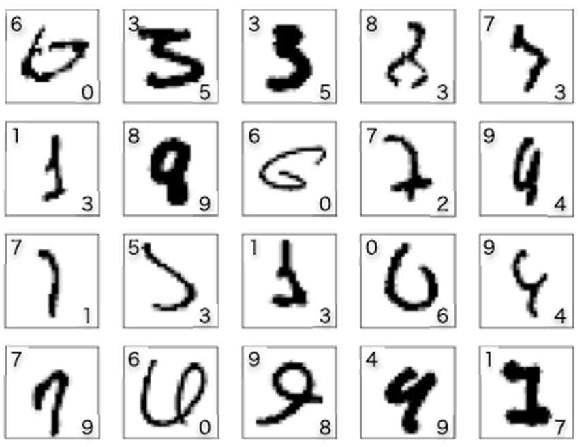
\includegraphics[width=0.6\columnwidth]{Fig_deep/Figure_2.pdf}
	\end{figure}
\end{frame}

\begin{frame}
	\frametitle{정확도를 더 높이려면}
	\begin{figure}
		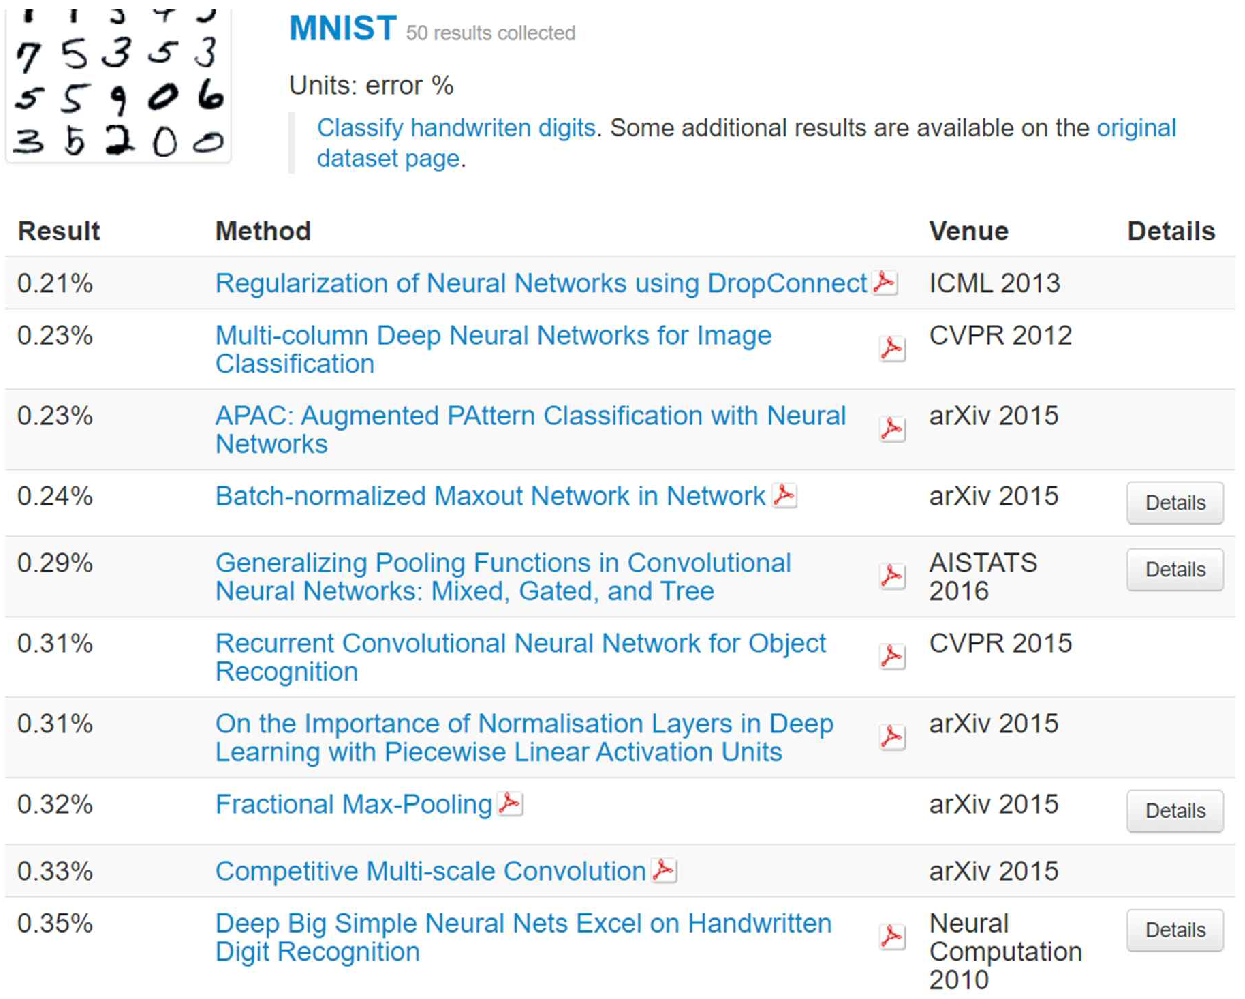
\includegraphics[width=0.7\columnwidth]{Fig_deep/Figure_3.pdf}
	\end{figure}
\end{frame}

\begin{frame}
	\frametitle{정확도를 더 높이려면}
	\begin{itemize}
		\item 상위권은 대부분 CNN 기초 한 기법
		\item CNN 기법들은 깊은 심층망이 아님(합성곱2개, 완전연결계층 2개)
		\item 앙상블 학습, 학습률 감소, 데이터 확장 등이 정확도 향상에 공헌함
		\item 데이터 확장은 손쉬운 방법이면서 정확도 개선에 효과적임
	\end{itemize}
\end{frame}

\begin{frame}
	\frametitle{데이터 확장}
	\begin{itemize}
		\item 입력 이미지를 알고리즘을 동원해 인위적으로 확장
		\item 입력 이미지를 회전하거나 세로로 이동하는 등 미세한 변화를 주어 이미지 개수 확장
		\item 데이터가 얼마 없을 경우 효과적인 수단
		\item crop(이미지를 잘라냄), flip(이미지를 좌우로 뒤집음), 스케일 변화
	\end{itemize}
	\begin{figure}
		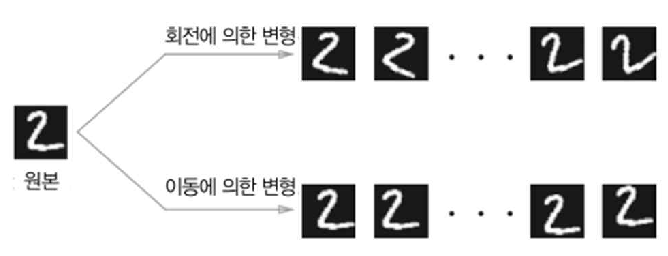
\includegraphics[width=0.7\columnwidth]{Fig_deep/Figure_4.pdf}
	\end{figure}
\end{frame}

\begin{frame}
	\frametitle{깊게하려는 이유}
	\begin{itemize}
		\item ILSVRC로 대표되는 대규모 이미지 인식 대회의 결과
		\item 매개변수가 줄어듬
		\item 적은 매개변수로 같은 수준의 표현력을 달성할 수 있음
	\end{itemize}
	\begin{figure}
		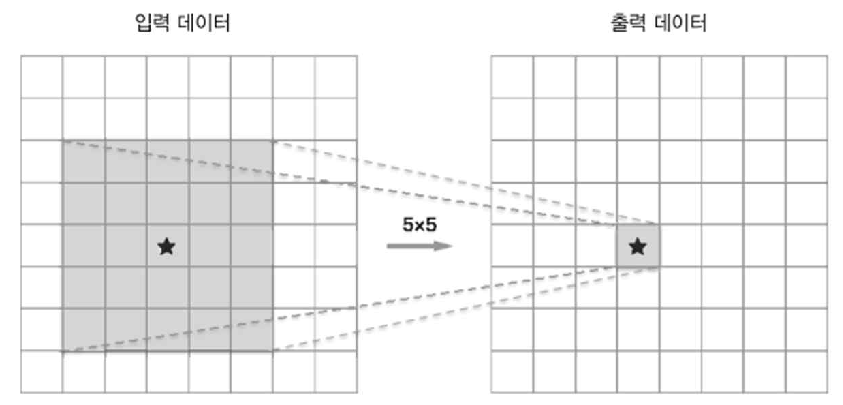
\includegraphics[width=1\columnwidth]{Fig_deep/Figure_5.pdf}
	\end{figure}
\end{frame}

\begin{frame}
	\frametitle{깊게하려는 이유}
	\begin{itemize}
		\item 학습해야 할 문제를 계층적으로 분해할 수 있음
		\item 각 층이 학습해야 할 문제를 더 단순한 문제로 대체할 수 있음
		\item 정보를 계층적으로 전달할 수 있음
		\item 엣지를 추출한 층의 다음 층은 엣지 정보를 쓸 수 있음
		\item 보다 고도의 패턴을 효과적으로 학습할 수 있음
	\end{itemize}
	\begin{figure}
		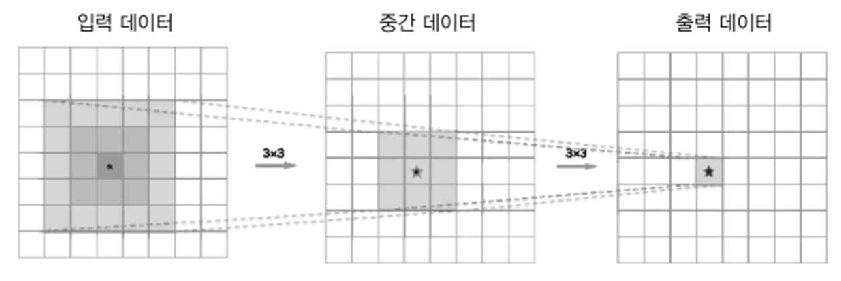
\includegraphics[width=1\columnwidth]{Fig_deep/Figure_6.pdf}
	\end{figure}
\end{frame}

\section{딥러닝의 초기 역사}
\begin{frame}
	\frametitle{이미지넷}
	\begin{itemize}
		\item 이미지넷은 100만장 넘는 이미지를 담고 있는 데이터셋
		\item ILSVRC는 이미지넷을 사용하여 이미지 인식 기술을 겨루는 대회를 개최
	\end{itemize}
\end{frame}

\begin{frame}
	\frametitle{VGG}
	\begin{itemize}
		\item 합성곱 계층과 풀링 계층으로 구성되는 기본적인 CNN
		\item 비중있는 층(합성곱 계층, 완전연결 계층)을 모두 16층으로 심화함
		\item 3*3의 작은 필터를 사용한 합성곱 계층을 연속으로 거침
	\end{itemize}
	\begin{figure}
		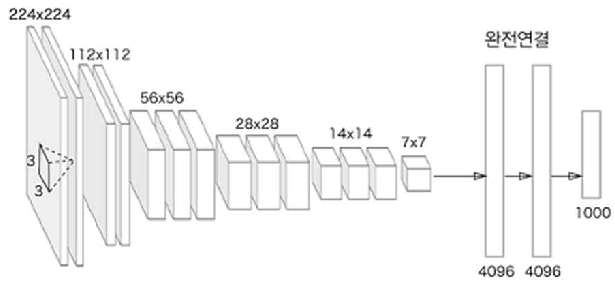
\includegraphics[width=0.8\columnwidth]{Fig_deep/Figure_7.pdf}
	\end{figure}
\end{frame}

\begin{frame}
	\frametitle{GoogLeNet}
	\begin{itemize}
		\item 가로방향에 폭이 있는 인셉션구조
		\item 인셉션구조는 크기가 다른 필터를 여러 개 적용하여 그 결과를 결합
		\item 1*1 채널을 줄여서 매개변수 제거와 고속처리에 기여함
	\end{itemize}
	\begin{figure}
		\subfigure{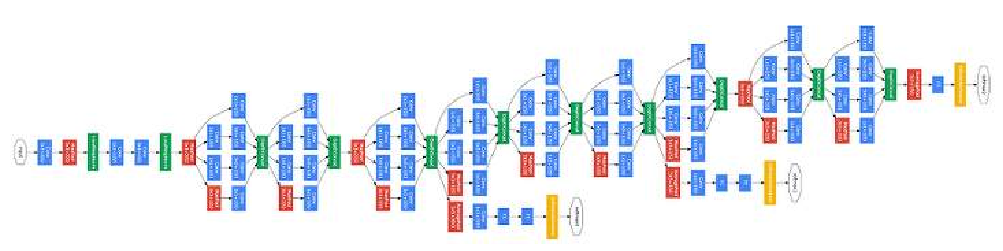
\includegraphics[width=0.5\columnwidth]{Fig_deep/Figure_8.pdf}}
		% \vspace{0.5cm}
		\subfigure{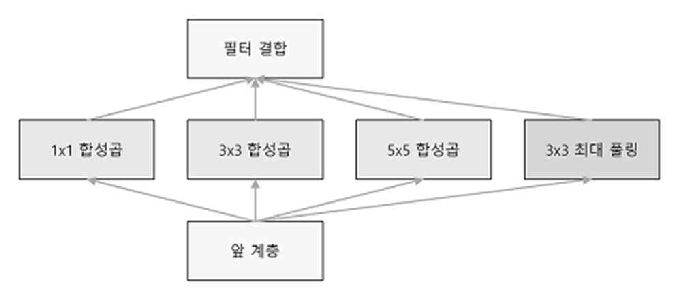
\includegraphics[width=0.3\columnwidth]{Fig_deep/Figure_9.pdf}}
	\end{figure}
\end{frame}

\begin{frame}
	\frametitle{ResNet}
	\begin{itemize}
		\item MS에서 개발한 CNN
		\item 층이 지나치게 깊어지면, 학습이 잘 안되어서 성능이 떨어지는 경우도 발생함
		\item 스킵 연결을 도입하여 층의 깊이에 비례해 성능을 향상 시킬 수 있음
	\end{itemize}
	\begin{figure}
		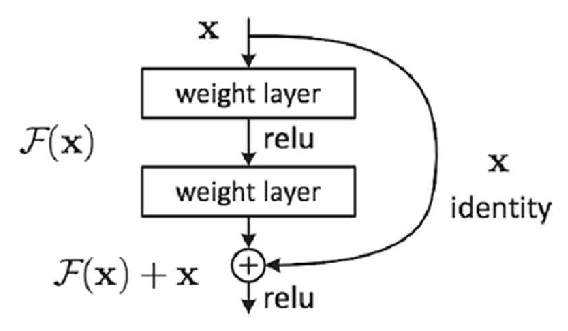
\includegraphics[width=0.5\columnwidth]{Fig_deep/Figure_10.pdf}
	\end{figure}
\end{frame}

\section{더 빠르게(딥러닝 고속화)}
	\begin{frame}
		\frametitle{풀어야 할 숙제}
		\begin{itemize}
			\item 딥러닝 처리 시간은 오랜시간을 합성곱 계층에서 소요
			\item GPU에서는 전체의 95\%, CPU에서는 89\% 사용
			\item 합성곱 계층의 연산을 어떻게 효율적으로 향상시킬까?가 딥러닝 네트워크의 핵심
		\end{itemize}
\end{frame}

\begin{frame}
	\frametitle{GPU를 활용한 고속화}
		\begin{itemize}
			\item 합성곱 계층은 대량의 단일 곱셈-누산을 수행함
			\item GPU는 병렬 수치 연산을 고속으로 처리할 수 있음
		\end{itemize}
\end{frame}

\begin{frame}
	\frametitle{분산학습}
		\begin{itemize}
			\item 딥러닝에서 발생하는 여러번의 시행착오 때문에 1회 학습에 걸리는 시간을 최대한 단축하려함
			\item 다수의 GPU와 컴퓨터를 이용한 분산학습 딥러닝 프레임워크 등장
			\item 텐서플로(구글), CNTK(마이크로소프트)
			\item 컴퓨터 사이의 통신과 데이터 동기화 등의 문제를 풀어야 함
		\end{itemize}
\end{frame}

\begin{frame}
	\frametitle{연산 정밀도와 비트 줄이기}
		\begin{itemize}
			\item 메모리 용량과 버스 대역폭 등이 딥러닝 고속화에 병목으로 발생
			\item 많은 비트를차지하는 실수연산은 메모리 사용량을 늘려 버스 대역폭에 부담을 줄 수 있음
			\item 딥러닝은 신경망의 견고성 때문에 높은 수치 정밀도를 요구하지 않음
			\item 딥러닝 고속화를 위해서 비트를 줄이는 기술이 필요함(임베디드용, Binarized Neural Networks)
		\end{itemize}
\end{frame}

\section{딥러닝의 활용}
\begin{frame}
	\frametitle{사물검출}
	\begin{itemize}
		\item 이미지 속에 담긴 사물의 위치와 종류를 알아내는 기술
		\item 후보영역 추출과 CNN으로 구분됨
	\end{itemize}
		\begin{figure}
			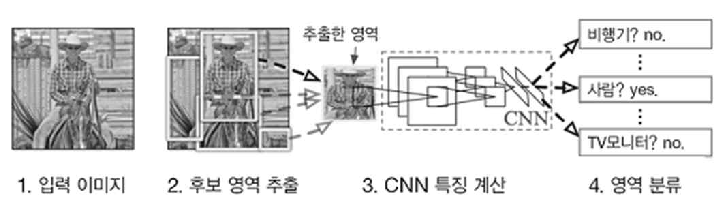
\includegraphics[width=0.8\columnwidth]{Fig_deep/Figure_11.pdf}
		\end{figure}
\end{frame}

\begin{frame}
	\frametitle{분할}
		\begin{itemize}
			\item 이미지를 픽셀 수준에서 분류
			\item 픽셀단위로 객체마다 채색된 지도 데이터를 사용해 학습
			\item 모든 픽셀을 대상으로 하나씩 추론 작업 실행
			\item FCN 기법을 이용하여 낭비를 줄여줌
		\end{itemize}
		\begin{figure}
			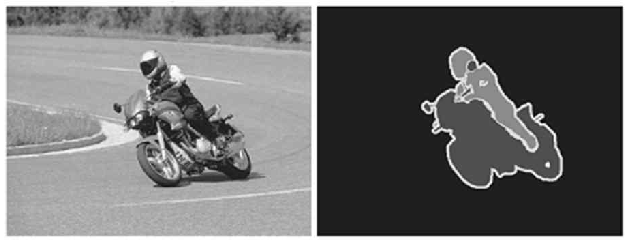
\includegraphics[width=0.8\columnwidth]{Fig_deep/Figure_12.pdf}
		\end{figure}
\end{frame}

\begin{frame}
	\frametitle{FCN}
		\begin{itemize}
			\item 합성곱 계층으로만 구성된 네트워크
			\item Forward 1회 처리만으로 모든 픽셀의 클래스를 분류함
			\item 공간 볼륨을 유지한 채 마지막 출력까지 처리함
			\item 이중 선형 보간법 사용
		\end{itemize}
		\begin{figure}
			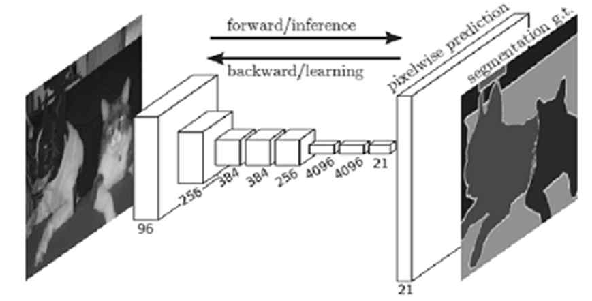
\includegraphics[width=0.8\columnwidth]{Fig_deep/Figure_13.pdf}
		\end{figure}
\end{frame}

\begin{frame}
	\frametitle{사진캡션생성}
	\begin{itemize}
		\item NIC(Neural Image Caption) : 심층 CNN + 자연어 순환신경망
		\item RNN : 자연어, 시계열 데이터 등의 연속된 데이터 처리
		\item Multimodal processing : 사진이나 자연어와 같은 여러 종류의 정보를 조합하여 처리
	\end{itemize}
\end{frame}

\section{딥러닝의 미래}
\begin{frame}
	\frametitle{이미지 스타일 변환}
		\begin{figure}
			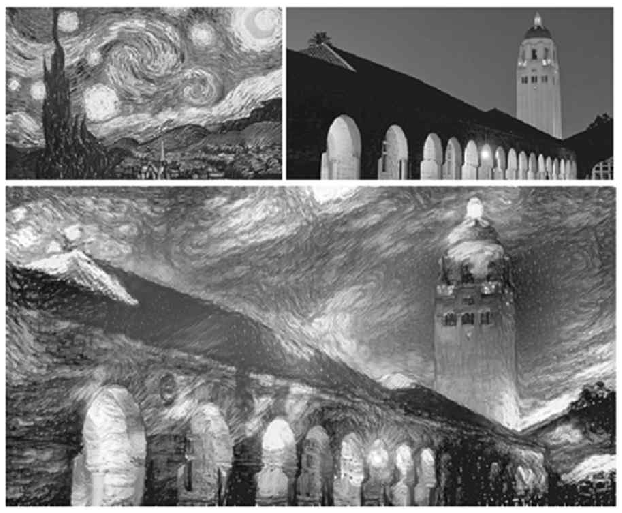
\includegraphics[width=0.6\columnwidth]{Fig_deep/Figure_14.pdf}
		\end{figure}
\end{frame}

\begin{frame}
	\frametitle{이미지생성}
		\begin{itemize}
			\item DCGAN(Deep Convolutional Generative Adversatial Network)
			\item 이미지를 생성하는 과정을 모델화
			\item 생성자(Generator)와 식별자(Discriminator)로 불리는 2개의 신경망 이용
			\item 생성자는 진짜 똑같은 이미지 생성
			\item 식별자는 이미지의 진위 판별
		\end{itemize}
\end{frame}

\begin{frame}
	\frametitle{자율주행}
		\begin{itemize}
			\item 안전한 주행 영역을 올바로 인식
			\item SegNet : CNN 기반 신경망
		\end{itemize}
		\begin{figure}
			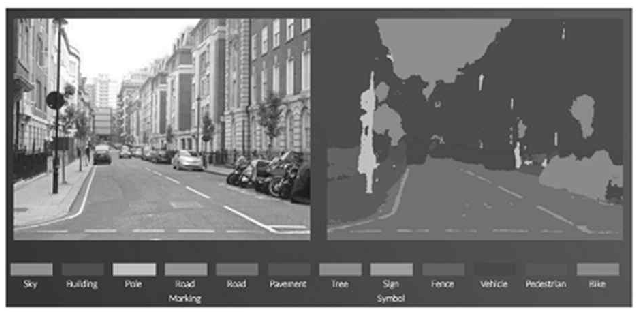
\includegraphics[width=0.8\columnwidth]{Fig_deep/Figure_15.pdf}
		\end{figure}
\end{frame}

\begin{frame}
	\frametitle{강화학습}
		\begin{itemize}
			\item 에이전트가 환경에 맞게 행동을 선택하여 환경이 변화함
			\item 환경 변화에 따라 에이전트가 보상을 받음
			\item 에이전트는 더 나은 보상을 받는 것이 목적임
			\item 최적 행동 가치 함수로 최적인 행동을 정하는 Q학습이라는 강화학습 알고리즘 이용
		\end{itemize}
		\begin{figure}
			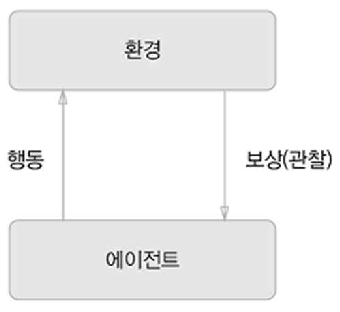
\includegraphics[width=0.3\columnwidth]{Fig_deep/Figure_16.pdf}
		\end{figure}
\end{frame}

\end{document}

